%        File: Intro.tex
%     Created: Sun Mar 02 03:00 PM 2014 P
% Last Change: Sun Mar 02 03:00 PM 2014 P
%
\documentclass[letterpaper,12pt]{article}
\usepackage[backend=bibtex]{biblatex}
\usepackage{fullpage}
\usepackage{hyperref}
\usepackage{amsmath}
\usepackage{graphicx}
%\usepackage[doublespacing]{setspace}
\addbibresource{CapstoneCitations.bib}

\pagestyle{plain}

\title{Humanoid Robotic Subsystems}
\date{April 14, 2014}
\author{Wenbo Wang \\University of California, Berkeley}

\begin{document}

\maketitle

\begin{abstract}
There is a growing need for manufacturing robots in many different sectors of
industry. As demand increases and technology improves there will be a great
demand for robots that can better integrate into the workplace. We propose two
new areas of Intellectual Property opportunities for Bay Area IP, LLC: Computer
Vision and Robotic Hands. There will be a great demand for robots that have high
precision and can better interact with human co-workers, as current
manufacturing robots are large machinery that are often not safe for human
workers. Computer vision allows the robot to be more aware of their surrounding,
and perform more tasks precisely. Humanoid hands also allow for more precision
and better integration with tools workspaces designed for humans. Are
preliminary results show great difficulty in building suitable robotic hands
with high dexterity without many the device large and cumbersome, but simple
computer vision can be built cheaply and effectively.  
\end{abstract}

\section{Introduction}
\paragraph{}Robots are being widely adopted by in many industries, and there is
a growing need for humanoid robotics. Humanoid robotic components can have many
applications such as manufacturing and prosthetics. A key component of our
project, the mechanical design of a humanoid robotic hand can be applied to both
manufacturing and prosthetics. Currently humanoid robots and robot subsystems
are not in wide use, so it is a good target for our sponsor, Bay Area IP, which
is looking do develop intellectual property that they could license to others.

\paragraph{}There are many technical challenges that come with trying to
reproduce the human form. The human body is very complex and there are many
different components that need to interact and function correctly. The human
hand has 27 degrees of freedom, and it is very difficult to reproduce that
complexity \cite{ElKoura2003}. However, modern manufacturing techniques such as
3D printing can get us closer to reproducing that complexity. Reproducing human
capabilities through software is also a great challenges. It is difficult to
design and implement complex control systems capable of mimicking the human
body. New computer hardware is allowing us to create more complex robots capable
of performing human like tasks.

\paragraph{}The subsystems we designed were the arms, hands, legs, feet, and
vision systems.  We designed the mechanical structure of these components and
the software for controlling the different parts. For the hands we did CAD
design of the hand structure. We also performed tests on using shape memory
alloy(SMA) to actuate components of in the fingers. Simple prototypes of the
arms and legs were constructed using off-the-shelf components to provide testing
platforms for the software. The control software was simulated in MATLAB and
then implemented in C++ on a microcontroller. The computer vision system was
implemented on an AMD APU, and utilized a novel laser system to augment the
computer vision algorithms.

\paragraph{}I was responsible for the construction of the mechanical arm, leg,
and the programming of the microcontroller. We implemented a simple control
algorithm for robot walking based on the Central Pattern Generator paradigm of
control.  This report will describe the materials and methods used to construct
the arms, and legs, as well as the programming of the microcontroller for basic
control of the robot. I will also give an overview of the other components of
the project.

\section{Literature Review}
\subsection{Computer Vision}
\paragraph{}Object detection has been well studied in a variety of applications.
Many machine learning algorithms are utilized for object detection such as
Support Vector Machines or Convolutional Neural
Networks\cite{Barbu2012},\cite{krizhevsky2012imagenet}. Many of the object
detection algorithms utilize Histogram of Oriented Gradient(HOG) features, which
are based on taking a gradient over the image and generating histograms of
gradient angles and magnitudes using overlapping sections of the
image\cite{Dalal2005}. 

\paragraph{}Complex object detection algorithms can be very resource intensive,
as they often need to scan the image multiple times at different resolutions to
find all the objects\cite{Felzenszwalb2013}. This can be a very expensive
process on an embedded system such as the robot. In a cluttered space it can be
very difficult to detect robots correctly in real time. On a robotic system
there usually exist other sensors that can supplement the visual information to
help ease this process. Utilization of depth sensors can help process the visual
information more easily\cite{Gould2008}.

\paragraph{}Computer vision techniques could have many applications for
manufacturing robots. As manufacturing robotics advance, they will need more
accuracy and intelligence to accomplish their tasks, and vision is a good tool
for accomplishing this. Already there are manufacturing robots utilizing vision
for tasks such as part recognition and sorting\cite{SIRfuture}.

\subsection{Robotic Hand}
\paragraph{}There are many different companies and research groups constructing
robotic hands for many different applications. There are hands designed to be
prosthetics, as well as hands designed to be integrated into robotic systems.
One of the most complex is the UB Hand IV, this hand is nearly the same as a
human hand in terms of capabilities. However, the hand is very heavy and very
power hungry, so it is not very suitable for most
applications\cite{Melchiorri2013}. However, most light weight hands are lacking
in complexity and function. The this recently developed lightweight hand only
has five degrees of freedom\cite{takaki2011high}. To develop a hand that is both
light weight, small, and fully functional will require new design techniques. 

\subsection{Shape Memory Alloy}
\paragraph{}We want to leverage some modern technology to make a robotic hand
that is smaller and light weight. One potential tool is Shape Memory Alloy
(SMA), a type of material that can expand or contract when
heated\cite{Schetky1982}. Many metallic alloys exhibit the shape memory
effect\cite{Wayman1993}. These alloys can be deformed at a lower temperature,
when heated, they will return to their original shape. We can use this do
accomplish actuation using a small form device heated through electrical
current\cite{Ikuta1990}. This actuation can be used in the fingers of the hand
, where space is very limited.

\subsection{Robot Leg}
\paragraph{}A popular control method for robot locomotion is Central Pattern
Generators (CPG). Central pattern generators are neural networks that generate
periodic control signals in the body. This control can be generated in the
absence of feedback signals. The human body utilizes this
system for many different rythmic motor functions that the body needs to
perform\cite{cpggeneral}. 

\paragraph{}Central pattern generator can also be adapted to the locomotion of
robots. CPG can be used to control locomotion of bipedal robots, as well as
hexapods and octopods. Using coupled oscillators one can design a control system
for bipedal robots. CPG are well suited for feedback control of bipedal
locomotion. Properly implemented CPG also allow for higher level control of the
walking without needing to worry about exact servo outputs. However CPGs are not
well understood and difficult to design properly\cite{Ijspeert2008}.

\subsection{Robot Arm}
\paragraph{}For the controls of our robot arm we will be implementing Fuzzy
Logic control systems. These control systems can handle nonlinearities well they
are well studied for control of robotic systems such as arms\cite{Scharf1985}.
Fuzzy logic controllers can also be used to control balance of the robotic legs,
treating the legs as an inverted pendulum\cite{hwang1992stability}.

\paragraph{}Rather than using complex models, a fuzzy logic controller relies on
empirical rules, this makes the controller computationally cheap and well suited
for embedded applications. A fuzzy logic controller has three main components: a
fuzzifier, a rule base, and an defuzzifier. In the fuzzifier, analog inputs are
fuzzified into fuzzy logic values between 0 and 1. The fuzzy values are put into
the rule base to determine a set of fuzzy outputs, and then the defuzzifier
combines the outputs into an analog output\cite{Mailah2000}.


\section{Materials and Methods}
\subsection{Materials}
\paragraph{PIC32MX795F512L:}A 32 bit micro-controller for performing the control
algorithms of the robot. The PIC32MX795F512L comes from SparkFun electronics as
part of the UBW32 board, which comes preloaded with a bootloader for programming
the board. See figure \ref{ubw32fig} for an image of the UBW32 board. The
PIC32MX795F512L is programmed in C/C++. To make the device easier to use, we
loaded an avrdude bootloader onto the device to use the MPIDE software. The
MPIDE framework allows us to use Arduino libraries on the PIC32MX795F512L which
helps to accelerate development of basic I/O software for the
board\cite{pic32data}.

\begin{figure}
  \centering
    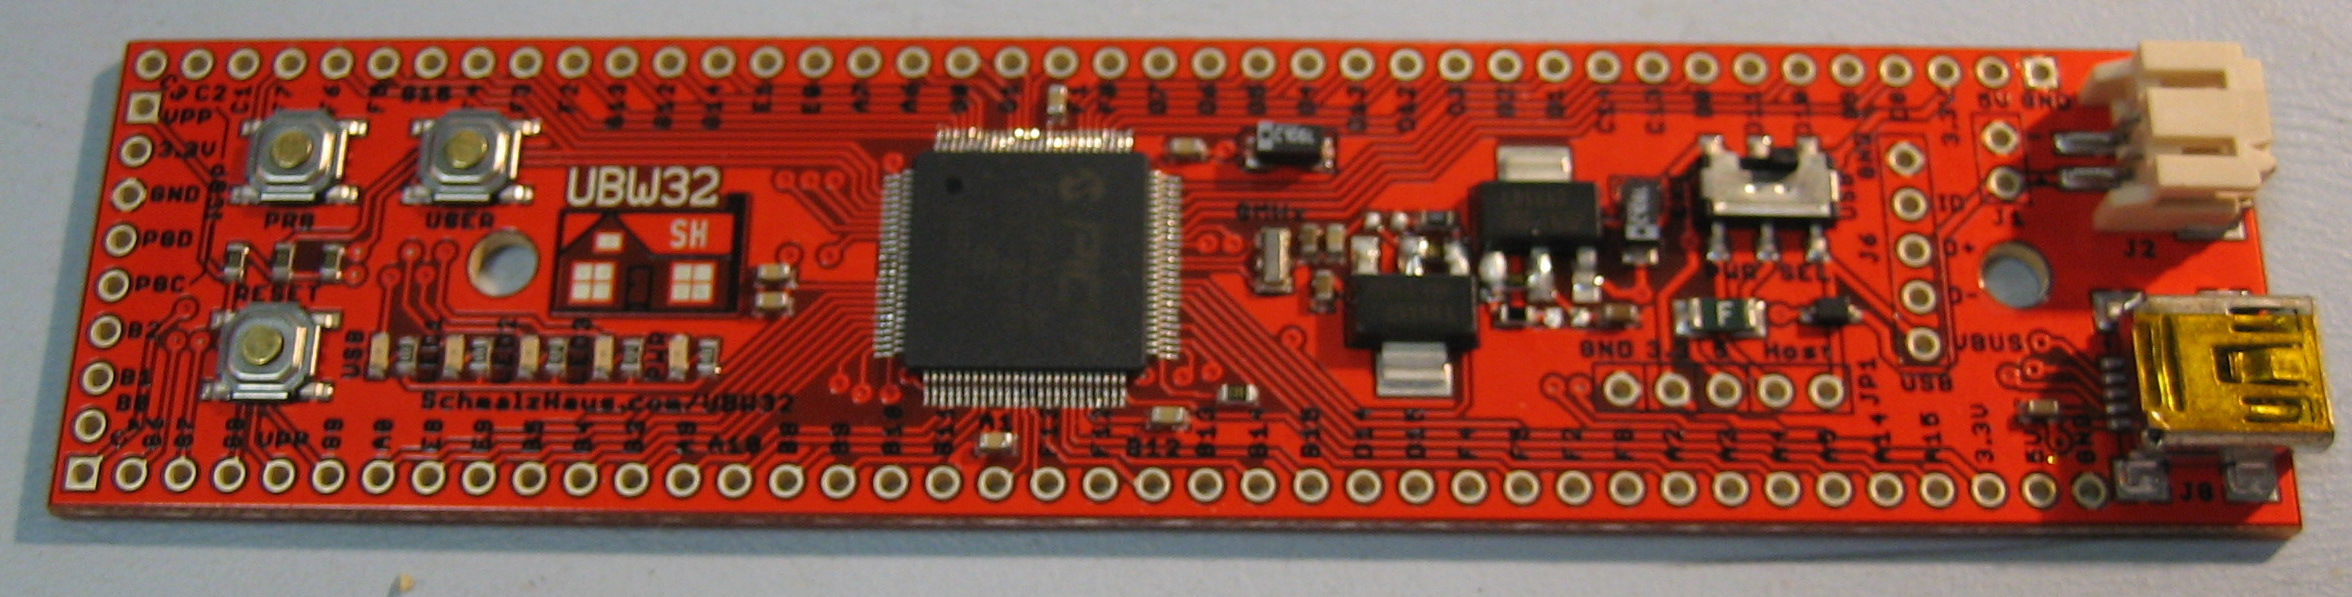
\includegraphics[width=0.75\textwidth]{figures/UBW32_v24_SparkFun.JPG}
  \caption{UBW32 board from SparkFun electronics}
  \label{ubw32fig}
\end{figure}

\paragraph{PICKIT3:}A hardware programmer for the PIC32MX795F512L
microprocessor. See figure \ref{pickit3fig}. The pickit3 and program and debug
the PIC32 micro-controller.  Used to download code onto the UBW32. Useful for
installing new bootloaders onto the UBW32 and for restoring broken
firmware\cite{pickitdata}.

\begin{figure}
  \centering
    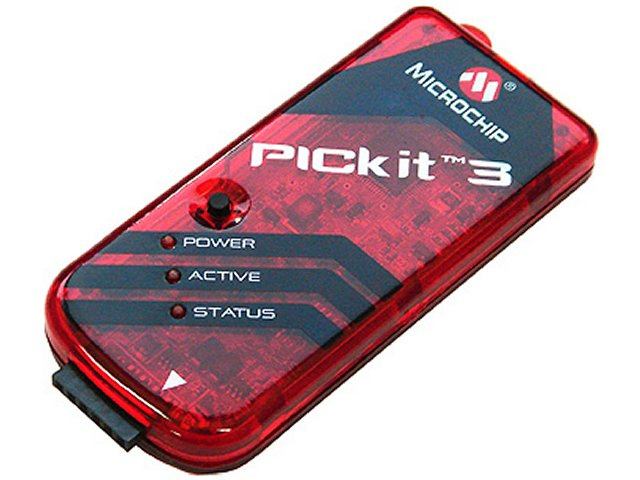
\includegraphics[width=0.3\textwidth]{figures/pickit3.jpg}
  \caption{PICkit 3 In-Circuit Debugger from Microchip}
  \label{pickit3fig}
\end{figure}

\paragraph{MPU6050:}A gyro and accelerometer for obtaining information about the
kinematics of the arm and the leg. See figure \ref{mpufig}. Uses I2C connection
to the PIC32MX795F512L for communication\cite{mpu6050data}.

\begin{figure}
  \centering
    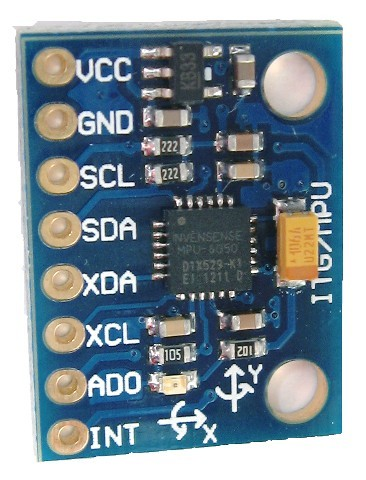
\includegraphics[width=0.2\textwidth]{figures/mpu-6050.jpg}
  \caption{MPU-6050 Triple axis accelerometer and gyro}
  \label{mpufig}
\end{figure}

\paragraph{HSR-5498SG:}Servos from Hitec. Utilized to control arm and leg
joints. See figure \ref{hsrfig}. The servos require 6-7 Volts. Each servo
requires at least 200mA when running without load, and over 1A when stalled.
The actuation of the arm is accomplished by mini-motors rather than
servos\cite{sscdata}.

\begin{figure}
  \centering
    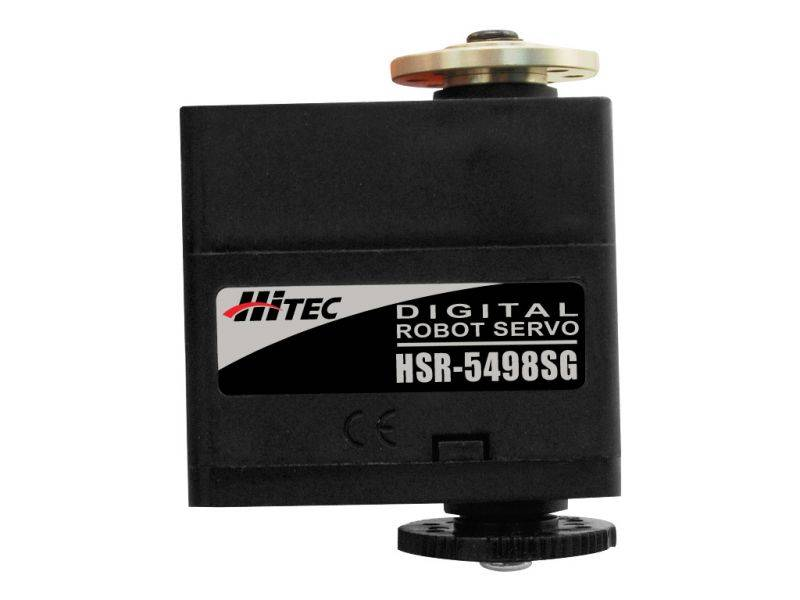
\includegraphics[width=0.4\textwidth]{figures/191_1_HSR-5498SG_HMI_Premium_Robot_Servo-1.jpg}
  \caption{HSR-5498SG servo from Hitech}
  \label{hsrfig}
\end{figure}

\paragraph{SSC-32:}Servo controller from Lynx motion. The on-board controller is
an Atmega168-20PU. See figure \ref{sscfig}. The SSC-32 is controlled using
serial signals from another microprocessor or the PC. The control signal is a
simple byte stream. The controller can specify pin number, servo position,
rotation speed, and rotation time. It can power 32 servos
simultaneously\cite{servodata}.

\begin{figure}
  \centering
    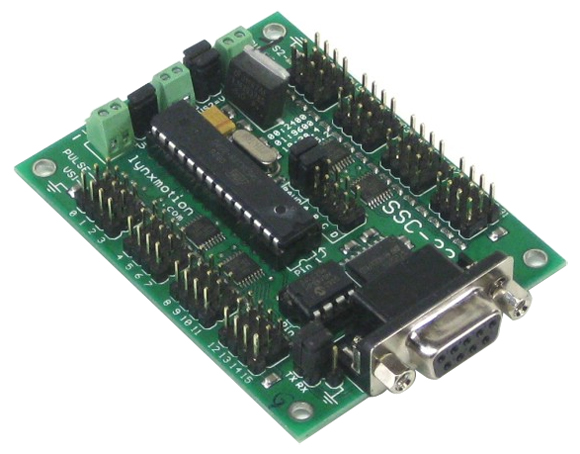
\includegraphics[width=0.4\textwidth]{figures/lynxmotion-ssc-32-servo-controller-large.jpg}
  \caption{SSC-32 servo controller from Lynxmotion}
  \label{sscfig}
\end{figure}

\paragraph{VLT100-4002}Power supply for powering the servos. See figure
\ref{vltfig}. 5V output capable of supplying 3A to 12A of current\cite{vltdata}.

\begin{figure}
  \centering
    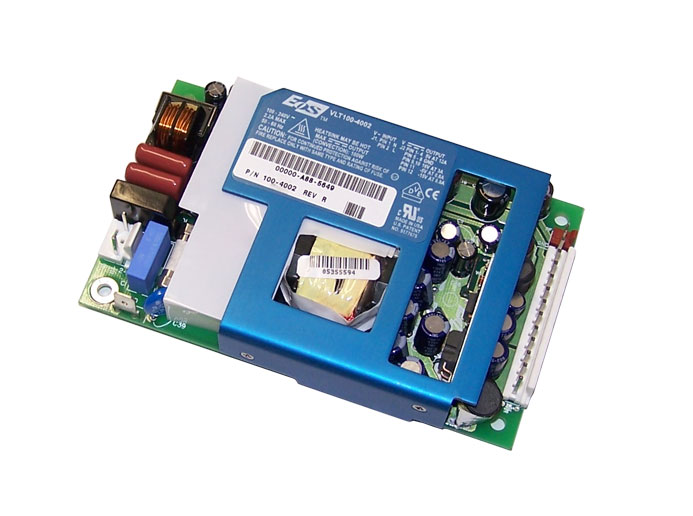
\includegraphics[width=0.4\textwidth]{figures/VLT100-4002.jpg}
  \caption{VLT100-4002 power supply}
  \label{vltfig}
\end{figure}

\paragraph{Yihua 1502DD}Adjustable power supply for servos. See figure
\ref{yihuafig}. 0-15V output and 0-2A output\cite{yihuadata}. 

\begin{figure}
  \centering
    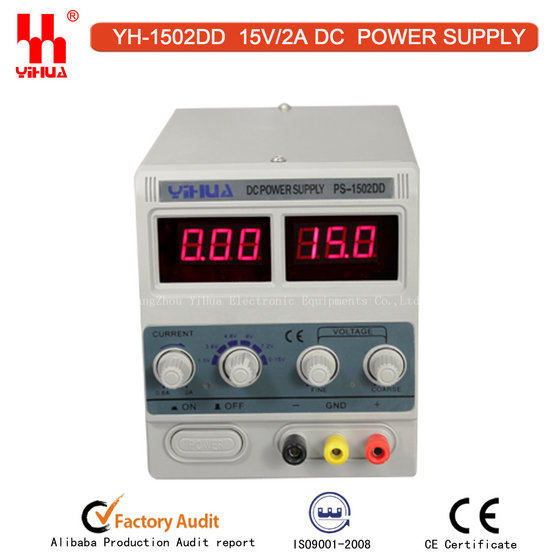
\includegraphics[width=0.4\textwidth]{figures/Power_Supply_YIHUA_1502DD.jpg}
  \caption{Yihua 1502DD DC power supply}
  \label{yihuafig}
\end{figure}

\subsection{Methods}
\subsubsection{Preliminary Setup}
\paragraph{}To program the PIC32MX795F512L, we used the Multi-Platform
Integrated Development Environment(MPIDE) environment from chipKIT. To use MPIDE
with the program, we had to program the PIC32 with the avrdude bootloader found
here: \url{https://github.com/chipKIT32/PIC32-avrdude-bootloader}. Using the
pickit3, we loaded the new bootloader onto the UBW32 and was able to use MPIDE
to program the board.

\paragraph{}While the other team members were constructing the mechanical
components of the legs and arms, I proceeded to set up the basic components of
the controller. We set up the MPU6050 using the PIC32 I2C libraries in MPIDE and
proceeded to do basic calibration and testing. Then we set up the servos using
the SSC-32 controller and the PIC32. Using the PIC32's Universal Asynchronous
Receiver/Transmitter(UART) we set up a serial communication channel between the
PIC32 and the SSC-32.  

\subsubsection{Servo Setup} 
\paragraph{} To control the servos we would send a string through the PIC32 UART
channel to the SSC-32. The string encoded the pin number, desired position and
desired rotation time for one of the 32 servo channels on the
SSC-32\cite{sscdata}. There were six servos on each leg of the robot and four on
each arm. On the legs, there were two servos per ankle, one on the knee, and
three on the hip. In total that gives us six degrees of freedom.  The arms were
assembled similarly, with one servo on the elbow and three in the shoulder. The
servos were powered through the SSC-32 board. Each servo requires around 200mA
of current and 6-7V of voltage\cite{servodata}. We used a 6V power supply to
power the servos channels on the SSC-32, and a 9V battery to power the logic
circuit of the servos. The PIC32 was powered through a USB connection to the PC.

\subsubsection{Walking Algorithm Implementation} 
\paragraph{} The walking algorithms were designed by Zhu Ziqi, a fellow team
member. He designed and simulated the algorithms in MATALB and SIMULINK and I
implemented the algorithms in C++ on the PIC32MX795F512L. The algorithms are
based on Central Pattern Generators, a part of biological neural networks which
generate rhythmic control signal for human motion\cite{cpggeneral}. The servos
are controlled using sine waves of varying shapes to generate patterns for
walking. Ziqi performed simulations to to select the best parameters for the
sine waves. For our preliminary walking algorithms we only considered the knee
and hip joints, keeping the other joints rigid. The SSC-32 position control
signal requires a integer ranged from 500 to 2500, corresponding to
$180^{\circ}$ of motion\cite{sscdata}. Due to the mechanical construction of the
arm and leg joints, which mimicked human structure, most joint servos were
limited to a range between 1250 and 2500. The output from the sine waves would
be converted to a range in the SSC-32's output and then sent to the servos. 
\begin{align}
    sine_{knee\_joint}=sin(eqn\_pending) \label{sineknee}\\
    sine_{hip\_joint}=sin(eqn\_pending) \label{sinehip}
\end{align}
Equations \ref{sineknee} and \ref{sinehip} show the equations for calculating
the position of each servo as a function of time. The positions of the legs are
calculated by the PIC32 and sent to the SSC-32.

\subsubsection{Leg Balance Algorithm}
%TODO: Get Yanchen's algorithms
\paragraph{} Waiting for team member to finish simulations of control
algorithms. Likely will use the MPU6050 to get the information about balance.

\subsubsection{Arm Control Algorithm}
\paragraph{} The arms are controlled using a Fuzzy Inference System. A fuzzy
inference system comprises of a fuzzifier, inference system, and defuzzifier.
The fuzzyfier takes inputs and out converts them to fuzzy values of a set of
fuzzy variables for the inference system. In this case the input is the desired
position of the arm in 3D space. The inference system is a set of if else
statements that determine a desired output from the fuzzy values. The
defuzzifier then converts this output to a real output to our
servos\cite{fuzzy2011}. To design this system we will take two approaches, one
through simulation and one through machine learning. I will work on the Machine
Learning approach. MATLAB has neural network algorithms that will generate fuzzy
inference systems. To do this we will generate a dataset based on the forward
kinematics of the robot arm, by giving it the angles of the arm joints and
calculating the arm position as a result of the joint angles. Inputing this
dataset into a machine learning framework in MATLAB, we can generate a simple
fuzzy inference system to control the robotic arm\cite{fuzzymatlab}. To further
refine the control algorithm, we will need to hand tune and simulate the fuzzy
inference system, as well as utilize gyro, accelerometer, and IR sensors to help
guide the arm and avoid obstacles.

\subsubsection{Computer Vision}
\paragraph{} To be completed\dots uses serial communication from APU to PIC32 to
transmit desired arm coordinates.

\subsubsection{Control of Hand}
\paragraph{} Not sure if implementation of hand control is needed for project.

\printbibliography

\end{document}
